\documentclass[12pt,a4paper,final]{beamer}
\usetheme{PaloAlto}

\usepackage[utf8]{inputenc}
\usepackage[portuguese]{babel}
\usepackage[T1]{fontenc}
\usepackage{graphicx}

\author{Warley Gonçalves dos Santos}
\title{Informática Básica Aula 1}
\institute{Associação Gesto de Amor}
\date{2018}
\logo{
\includegraphics[scale=0.058]{imagens/logo.jpg}}

\begin{document}
% Page 1
	\begin{frame}
		\titlepage
	\end{frame}

% Page 2
    \begin{frame}
        \frametitle{O que é Informática?}
        \framesubtitle{Concepção}
        \begin{block}{Origem da palavra:}
            Em 1956, o cientista da computação alemão \textbf{Karl Steinbuch} publicou o periódico:
        \end{block}
        \begin{block}{}
             \centering
             \emph{\textbf{Informática:} Processamento Automático de Informação}
             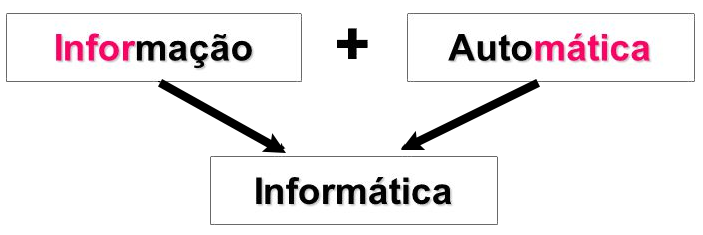
\includegraphics[scale=0.3]{Imagens/informatica.png}
        \end{block}
	\end{frame}
% Page 3
    \begin{frame}
        \frametitle{O que é Informática?}
        \framesubtitle{Pirâmide do Conhecimento}
        \begin{block}{}
             \centering
             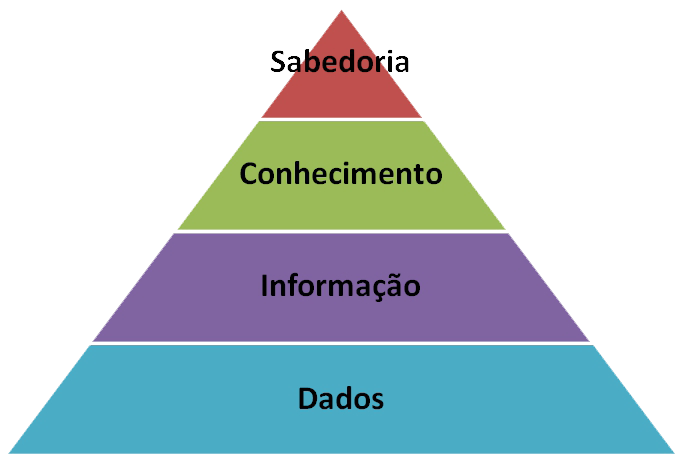
\includegraphics[scale=0.5]{Imagens/piramede.png}
        \end{block}
	\end{frame}
\end{document}